\documentclass[9pt]{beamer}
\usetheme[faculty=fi]{fibeamer}
\usepackage[T2A]{fontenc}
\usepackage[utf8]{inputenc}
\usepackage[
  main=ukrainian, %% By using `czech` or `slovak` as the main locale
                %% instead of `english`, you can typeset the
                %% presentation in either Czech or Slovak,
                %% respectively.
  english, russian %% The additional keys allow foreign texts to be
]{babel}        %% typeset as follows:
%%
%%   \begin{otherlanguage}{czech}   ... \end{otherlanguage}
%%   \begin{otherlanguage}{slovak}  ... \end{otherlanguage}
%%
%% These macros specify information about the presentation
\title{Криптосистеми на еліптичних кривих} %% that will be typeset on the
%\subtitle{Presentation Subtitle}
\subtitle{Lecture 4: Forms}

\author{Грубіян Євген Олександрович}

%% These additional packages are used within the document:
\usepackage{ragged2e}  % `\justifying` text
\usepackage{booktabs}  % Tables
\usepackage{tabularx}
\usepackage{tikz}      % Diagrams
\usetikzlibrary{calc, shapes, backgrounds}
\usepackage{amsmath, amssymb}
\usepackage{url}       % `\url`s
\usepackage{listings}  % Code listings
\usepackage{wrapfig}
\frenchspacing
\begin{document}
  \frame{\maketitle}


  \begin{darkframes}
      
    \section{Light Frames}


%%%%%%%%%%%%%%%%%%%%%%%%%%%%%%%%%%%%%%%%%%%%%%%%%%%%%%%%%%%%%%%%%%%%%%%%%%%%%%
% Слайди 1-3: Відображення між еліптичними кривими: ізоморфізми, ендоморфізми, ізогенії
%%%%%%%%%%%%%%%%%%%%%%%%%%%%%%%%%%%%%%%%%%%%%%%%%%%%%%%%%%%%%%%%%%%%%%%%%%%%%%

\section{Відображення між еліптичними кривими}
\begin{frame}{Ізоморфізм}

\begin{block}{Ізоморфізм еліптичних кривих}
    Біраціональне відображення $\phi: E \longrightarrow E'$ між двома еліптичними кривими, що зберігає групову структуру(ізоморфізм їх груп), а також $\phi(\mathcal{O}_E)=\mathcal{O}_{E'}$
\end{block}
Якщо криві задані в формі Вейєрштраса
\[
  E/K: \quad y^2 = x^3 + ax +b, \qquad
  E'/K: \quad y^2 = x^3 + a'x + b'.
  \]
  Тоді всі біраціональні відображення що зберігають групову структуру (ізоморфізми) можна задати:
\[
  a' = u^4 a, \quad b' = u^6 b \quad \phi(x,y) = (u^2 x,\, u^3 y)
  \]
  Де $u \in \overline{K}$, при чому воно єдине для 2х ізоморфних кривих
\end{frame}

\begin{frame}{\(j\)-інваріант еліптичної кривої}
  \begin{block}{\(j\)-інваріант}
    Нехай \(E/K: y^2 = x^3 + ax + b\) --- еліптична крива у формі Вейєрштраса.
    Тоді \(j\)-інваріант \(E\) визначається як
    \[
    j(E) = 1728\,\frac{4a^3}{4a^3+27b^2}.
    \]
  \end{block}
  
  \begin{itemize}
    \item Еліптичні криві \(E/K\) та \(E'/K\) є ізоморфними тоді й тільки тоді, коли
      \[
      j(E) = j(E').
      \]
    \item Таким чином, \(j\)-інваріант класифікує класи ізоморфних еліптичних кривих, тобто задає відношення еквівалентності на множині еліптичних кривих над полем $K$.
  \end{itemize}
\end{frame}


\begin{frame}{Криві кручення (Twists)}
  \begin{block}{Крива кручення}
    Нехай \(E/K: y^2=x^3+ax+b\) — еліптична крива. Еліптична крива \(E'/K\) називається \emph{кривою кручення} (twist) від \(E\), якщо існує ізоморфізм
    $
    \phi: E \rightarrow E'
    $
    визначений над алгебраїчним замиканням \(\overline{K}\), але \(\phi\) не визначений над \(K\).
  \end{block}
  \begin{block}{Квадратичне кручення (Quadratic Twist)}
    Якщо \(d\in K^\times\) є елементом, який не є квадратичним лишком в \(K\), тоді \emph{крива квадратичного кручення} \(E\):
    \[
    E^d/K: \quad d\,y^2 = x^3 + Ax + B,
    \]

    Криві \(E\) та \(E^d\) стають ізоморфними над \(K(\sqrt{d})\), але не ізоморфними над \(K\).
  \end{block}
  \textbf{Зауваження:} \(j\)-інваріанти задовольняють \(j(E)=j(E^d)\), тому криві з однаковим \(j\)-інваріантом можуть бути не ізоморфними над \(K\), а лише над \(\overline{K}\).
\end{frame}

\begin{frame}{Типи кручень еліптичних кривих}
  \begin{block}{Група автоморфізмів еліптичної кривої}
    Нехай \(E/K\) --- еліптична крива. 
    Група \(\operatorname{Aut}(E)\) складається з усіх біраціональних відображень (ізоморфізмів) 
    $
    \phi: E \to E,
    $

  \end{block}
  \textbf{Основні типи кручень:}
  \begin{itemize}
    \item \textbf{Квадратичні кручення:} Якщо \(j(E) \neq 0, 1728\), то \(\operatorname{Aut}(E)  \cong \{\pm 1\} \cong \mathbb{Z}/2\mathbb{Z}\), і всі кручення є квадратичними. 
    \item \textbf{Кубічні/секстичні кручення:} Якщо \(j(E)=0\), то \(\operatorname{Aut}(E) \cong \mu_6 \cong \mathbb{Z}/6\mathbb{Z}\) (група 6-их коренів одиниці). У цьому випадку, криві можуть мати кубічні або секстичні кручення.
    \item \textbf{Квартові кручення:} Якщо \(j(E)=1728\), то \(\operatorname{Aut}(E) \cong \mu_4 \cong \mathbb{Z}/4\mathbb{Z}\) (група 4-их коренів одиниці), тобто можуть існувати квартові кручення
  \end{itemize}

  \textbf{Зауваження:} Інших кручень не існує. Для більшості кривих визначені лише квадратичні кручення.
\end{frame}


%%%%%%%%%%%%%%%%%%%%%%%%%%%%%%%%%%%%%%%%%%%%%%%%%%%%%%%%%%%%%%%%%%%%%%%%%%%%%%
% Слайди 4-6: Форми еліптичних кривих: Montgomery, Edwards та їх еквівалентність
%%%%%%%%%%%%%%%%%%%%%%%%%%%%%%%%%%%%%%%%%%%%%%%%%%%%%%%%%%%%%%%%%%%%%%%%%%%%%%

\section{Форми еліптичних кривих та їх ізоморфізми}
\begin{frame}{Форми еліптичних кривих}
  Сучасна криптографія використовує різні подання еліптичних кривих. Серед них:
  \begin{itemize}
    \item \textbf{Форма Вейєрштраса:} \( E_w/K: y^2 = x^3 + ax + b \).
    \item \textbf{Форма Монтомері:} \( E_m/K: B\, y^2 = x^3 + A x^2 + x \).
    \item \textbf{Форма Едвардса:} \( E_d/K : a x^2 + y^2 = 1 + d x^2 y^2 \).
  \end{itemize}
  За певних умов ці форми є біраціонально еквівалентними. 
  \begin{itemize}
      \item Перехід $E_w \rightarrow E_m$ можливий якщо $\exists P\in E_w: ord(P)=2$
      \item Перехід $E_m \rightarrow E_w$ можливий завжди
      \item Перехід $E_d \leftrightarrow E_m$ можливий завжди в обидві сторони
  \end{itemize}
\end{frame}

\begin{frame}{Перехід від форми Вейєрштраса до форми Монтомері}
  \textbf{Вихідна форма (Вейєрштраса):}  
  $
  E_w/K: \quad y^2 = x^3 + ax + b.
  $
  
  \textbf{Умова:}  
  Для перетворення необхідно, щоб крива мала раціональну точку порядку 2, тобто існував \(r\in K\) та \(r^3+ar+b=0\) (тобто точка \(P=(r,0) \in E(K)\)).
  \begin{enumerate}
      \item Факторизуємо кубічний многочлен:
  $
  x^3 + ax + b = (x - r)(x^2 + cx + d).
  $
  \item Здійснюємо трансляцію змінної:
  $
  x = X + r, \quad y = Y.
  $
  Тоді рівняння набуває вигляду:
  \[
  Y^2 = X^3 + 3r X^2 + (3r^2+a)X,\quad \lambda=\sqrt{3r^2+a}
  \]
  \item Виконавши масштабування змінних отримаємо $ E_m/K: (1/\lambda ^3)Y^2 = X^3+(3r/\lambda)X^2 + X$
  \end{enumerate}
  

\end{frame}

\begin{frame}{Форма Монтомері та диференціальне додавання точок}
  Розглянемо еліптичну криву в формі Монтомері:
  \[
  E_m/K: B\,y^2 = x^3 + A\,x^2 + x \quad \Delta= B(A-4)\neq 0
  \]

  Однією з ключових властивостей цієї форми є диференціальне додавання: якщо маємо дві точки \(P\) та \(Q\), а також точку \(P-Q\) (різницю точок), то \(x\)-координата суми \(P+Q\) визначається лише через \(x\)-координати \(P\), \(Q\) та \(P-Q\).
  
  Наприклад, в афінних координатах (за певною нормалізацією) формула має вигляд:
  \[
  x(P+Q) = \frac{\Bigl(x(P)x(Q) - x(P-Q)\Bigr)^2}{\Bigl(x(P)-x(Q)\Bigr)^2}.
  \]
  

  \textbf{Перевага:}  
  Така властивість дозволяє реалізувати алгоритм \emph{Montgomery ladder} для скалярного множення, де обчислення проводяться лише над \(x\)-координатами, що підвищує ефективність і стійкість до side-chanel атак.
\end{frame}


\begin{frame}{Перехід від форми Монтгомері до форми Едвардса}
  Розглянемо криву в формі Монтгомері:
  \[
  E_m/K: \quad B\,y^2 = x^3 + A\,x^2 + x,
  \]

  Тоді відповідна крива у формі Едвардса записується як:
  \[
  E_d: \quad a\,x_E^2 + y_E^2 = 1 + d\,x_E^2y_E^2, \quad
  a = \frac{A+2}{B},\quad d = \frac{A-2}{B}.
  \]

  З наступним перетвореннями координат (за деякими виключеннями особливих точок порядків 2,4 та $\mathcal{O}$):
  \[
  x_E = \frac{x_M}{y_M},\quad
  y_E = \frac{x_M-1}{x_M+1},
  \]
  де \((x_M,y_M)\) --- координати на кривій \(E_M\).

  Зворотні перетворення:
  \[
  x_M = \frac{1+y_E}{1-y_E},\quad
  y_M =\frac{1}{x_E(1-y_E)}.
  \]
  
\end{frame}


%%%%%%%%%%%%%%%%%%%%%%%%%%%%%%%%%%%%%%%%%%%%%%%%%%%%%%%%%%%%%%%%%%%%%%%%%%%%%%
% Слайди 7-8: Арифметика в загальній формі Едвардса та її переваги
%%%%%%%%%%%%%%%%%%%%%%%%%%%%%%%%%%%%%%%%%%%%%%%%%%%%%%%%%%%%%%%%%%%%%%%%%%%%%%

\begin{frame}{Арифметика кривих в формі Едвардса}
  Нехай \(E_d\) --- крива в формі Едвардса
  \[
  E_d/K:a x^2 + y^2 = 1 + d x^2 y^2, \quad a \neq 0, d\neq0, d\neq a
  \]

  \textbf{Переваги цієї форми:}
  \begin{itemize}
    \item \textbf{Уніфікованість закону додавання:} Формули додавання та подвоєння мають єдиний вигляд і деколи є повними (без виключень). Точка на нескінченності переходить в $\mathcal{O} \rightarrow (0,1)$
    \item \textbf{Ефективність обчислень:} Криві Едвардса швидші в порівнянні з аналогами, зокрема існує ряд кривих, арифметика на яких є найшвидшою в класі (Ed25519).
    \item \textbf{Безпека:} Зменшена ймовірність виникнення виняткових випадків, що покращує захист від атак через витік інформації (наприклад, через аналіз сторони каналу).
  \end{itemize}
\end{frame}

\begin{frame}{Формули додавання  на кривих Едвардса}
  Нехай \(P=(x_1,y_1)\) та \(Q=(x_2,y_2)\) --- точки на кривій Едвардса
  \[
  E_d/K:a x^2+y^2 = 1+d x^2y^2.
  \]
  Тоді формули додавання мають вигляд:
  \[
  x_3 = \frac{x_1y_2 + y_1x_2}{1+d x_1x_2y_1y_2},\qquad
  y_3 = \frac{y_1y_2 - a x_1x_2}{1-d x_1x_2y_1y_2}.
  \]
\begin{center}
    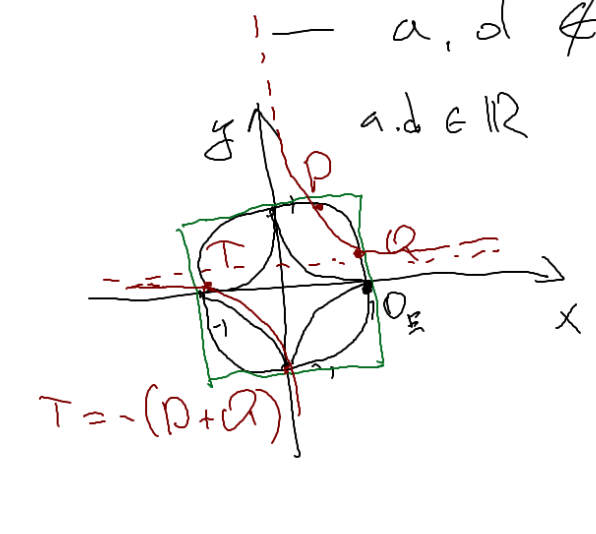
\includegraphics[width=0.5\textwidth]{resources/ed.png}
    \end{center}

\end{frame}

%%%%%%%%%%%%%%%%%%%%%%%%%%%%%%%%%%%%%%%%%%%%%%%%%%%%%%%%%%%%%%%%%%%%%%%%%%%%%%
% Завершальний слайд
%%%%%%%%%%%%%%%%%%%%%%%%%%%%%%%%%%%%%%%%%%%%%%%%%%%%%%%%%%%%%%%%%%%%%%%%%%%%%%
\begin{frame}{Класифікація кривих в формі Едвардса}
  Нехай \(E_d\) --- крива в формі Едвардса над $K$
  \[
  E_d/K:a x^2 + y^2 = 1 + d x^2 y^2, \quad a \neq 0, d\neq0, d\neq a
  \]
  $$QR(K)=\{x\in K^* | \exists y: y^2=x\}$$
  \begin{itemize}
    \item $ad\notin QR(K)$ - повні криві в формі Едвардса, завжди можна знайти ізоморфну криву із $a=1$. Особливі точки відсутні.
    \item $a,d\in QR(K)$ - квадратичні криві в формі Едвардса. Можуть існувати особливі точки порядку 2 або 4.
    \item $a,d\notin QR(K)$ - скручені криві в формі Едвардса. Можуть існувати особливі точки порядку 2.
  \end{itemize}
  
\end{frame}


  \end{darkframes}




\end{document}
